\newcommand{\pluginName}{Dates Generator}
\newcommand{\pluginVersion}{1.0}


\input{../../DocumentationTemplate/TemplateL2}

\section{Introduction}
Dates generator allows to generate a sequence of (payment) dates by specifying Starting Date, Ending Date and the frequency.  Dates can then be manipolated manually and trasformed with adjustments.
\section{How to use the plug-in}
In the new symbol dialog window, a new symbol type is available.

After Dates Generator has been installed as a plugin from ``Settings --> Plugins Settings 
-->Available online plugins'', you can use it select : 
\begin{enumerate}
\item Parameters \& Function;
\item Add;
\item Dates Generator.
\end{enumerate}
As you can see into the figure \label{fig:DG}, is possible set the start date and the end date setting also the right interval in months term, into the gap. 
\begin{figure}[h!]
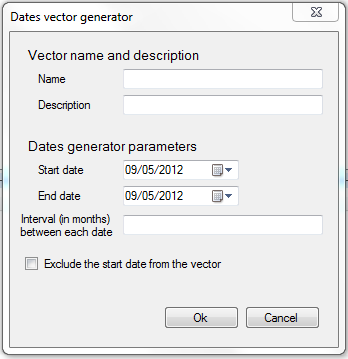
\includegraphics[width=4cm]{DG_img}
\centering
%\leftskip=-1.5 cm
\caption{\small{\emph{Dates Generator window.}}}
\label{fig:DG}
\end{figure}
Also, is possible to esclude the first date of the series.\\
\\
This new features allows to build a vector of date directly in Fairmat avoiding the 
copy and paste from other software (i.e. Excel spreadsheet).

\end{document}


